\subsection{DDPG with different noise processes}
\paragraph{Pendulum-v1}
The Pendulum-v1 environment was used for benchmarking in the early stages of the project. I first trained a DDPG agent with Gaussian noise and then added Ornstein-Uhlenbeck (OU) noise as an alternative, following the original DDPG paper \cite{ddpg_original}. With both noise processes, the agent quickly and consistently learned to balance the pendulum upright while maximizing rewards without excessive swinging.
Encouraged by promising results on exploration in continuous environments using pink noise \cite{eberhard2023pink}, I implemented a third noise process following the suggested process where \(\beta = 1\). However, the DDPG agent with pink noise failed to solve the Pendulum-v1 environment. This was likely due to the hyperparameter configuration I used for the noise process, which made the actions unstable after noise was added. As a result, the agent was unable to learn the correct rotation to keep the pendulum upright. The different noise processes can be found in the ´noise.py´ file under ´src/utils´ in our codebase.

\paragraph{Hockey-Env} 
In the Hockey environment, DDPG with all noise options struggled to outperform the strong bot, achieving only a 35 \% win rate after 2-3 hours of training on a GTX 1080 Ti GPU when using OU noise. Tuning noise-related hyperparameters like $\theta$ and $\sigma$ proved challenging. A few days before the competition, I decided to avoid the challenge of manually tuning exploration noise in deterministic RL agents. Instead, I switched to training a second algorithm that incorporates stochasticity directly in its policy design: the Soft Actor-Critic algorithm. This approach naturally includes noise as part of the stochastic policy, eliminating the need for manually adding exploration noise.

\subsection{SAC}
Due to time constraints the SAC agent is only tested on the Hockey Env. Reaching up to 66 percent win rate against bot strong after training against it for approximately 3 to 4 hours on a 1080ti GPU. I achieved this using the following hyperparameter configuration during training.

\paragraph{Configuration of hyperparameters and design choices}
The actor and both critic networks follow a 3 layer dense architecture with hiddensize of 400 and non linear ReLU activation. The target entropy that contributes to the temperature update was set to $-\text{dim}(\textit{action-space}) = -4$ for the hockey env controlling a single agent. The initial temperature controlling alpha was set to $\alpha = 0.2$. With $\gamma = 0.99$ we enable learning for long range future rewards to be important as well (very important for the hockey env due to its single non-zero reward of $10$ or $-10$ in case a goal is scored). The soft target update coefficiant which controls the rate at which the target networks slowly track the learned networks and thus playing a crucial role in training stability was first set to $\tau = 0.005$ and at later training stages set to $\tau = 0.0025$. All actor, critic and alpha optimizer learning rates were set to the default $0.0001$. Please refer to the codebase for more details.

\paragraph{Results}
This results section refers to the checkpoint used during the competition with name SigmaZero-SAC. After the warm-up phase, the alpha values stabilized around zero (see \ref{fig:alphas}), which is essential for stable learning in SAC. Meanwhile, the running average reward against the strong bot continued to rise, suggesting that convergence had not yet been reached. This indicates that with further training, the agent could have achieved even higher rewards and win rates during evaluation. For a visualization of the running average reward (computed over a window of 100) during training against the weak bot, please refer to Figure \ref{fig:rewards_sac}. Finally, evaluating 100 games many times with the deterministic action selection yields a win rate of $65\pm5 \ \%$ as shown for one evaluation run with 100 games in figure \ref{fig:wins_sac}.
\begin{figure}[htbp]
    \centering
    \subfloat[Smoothed reward over the training episodes]{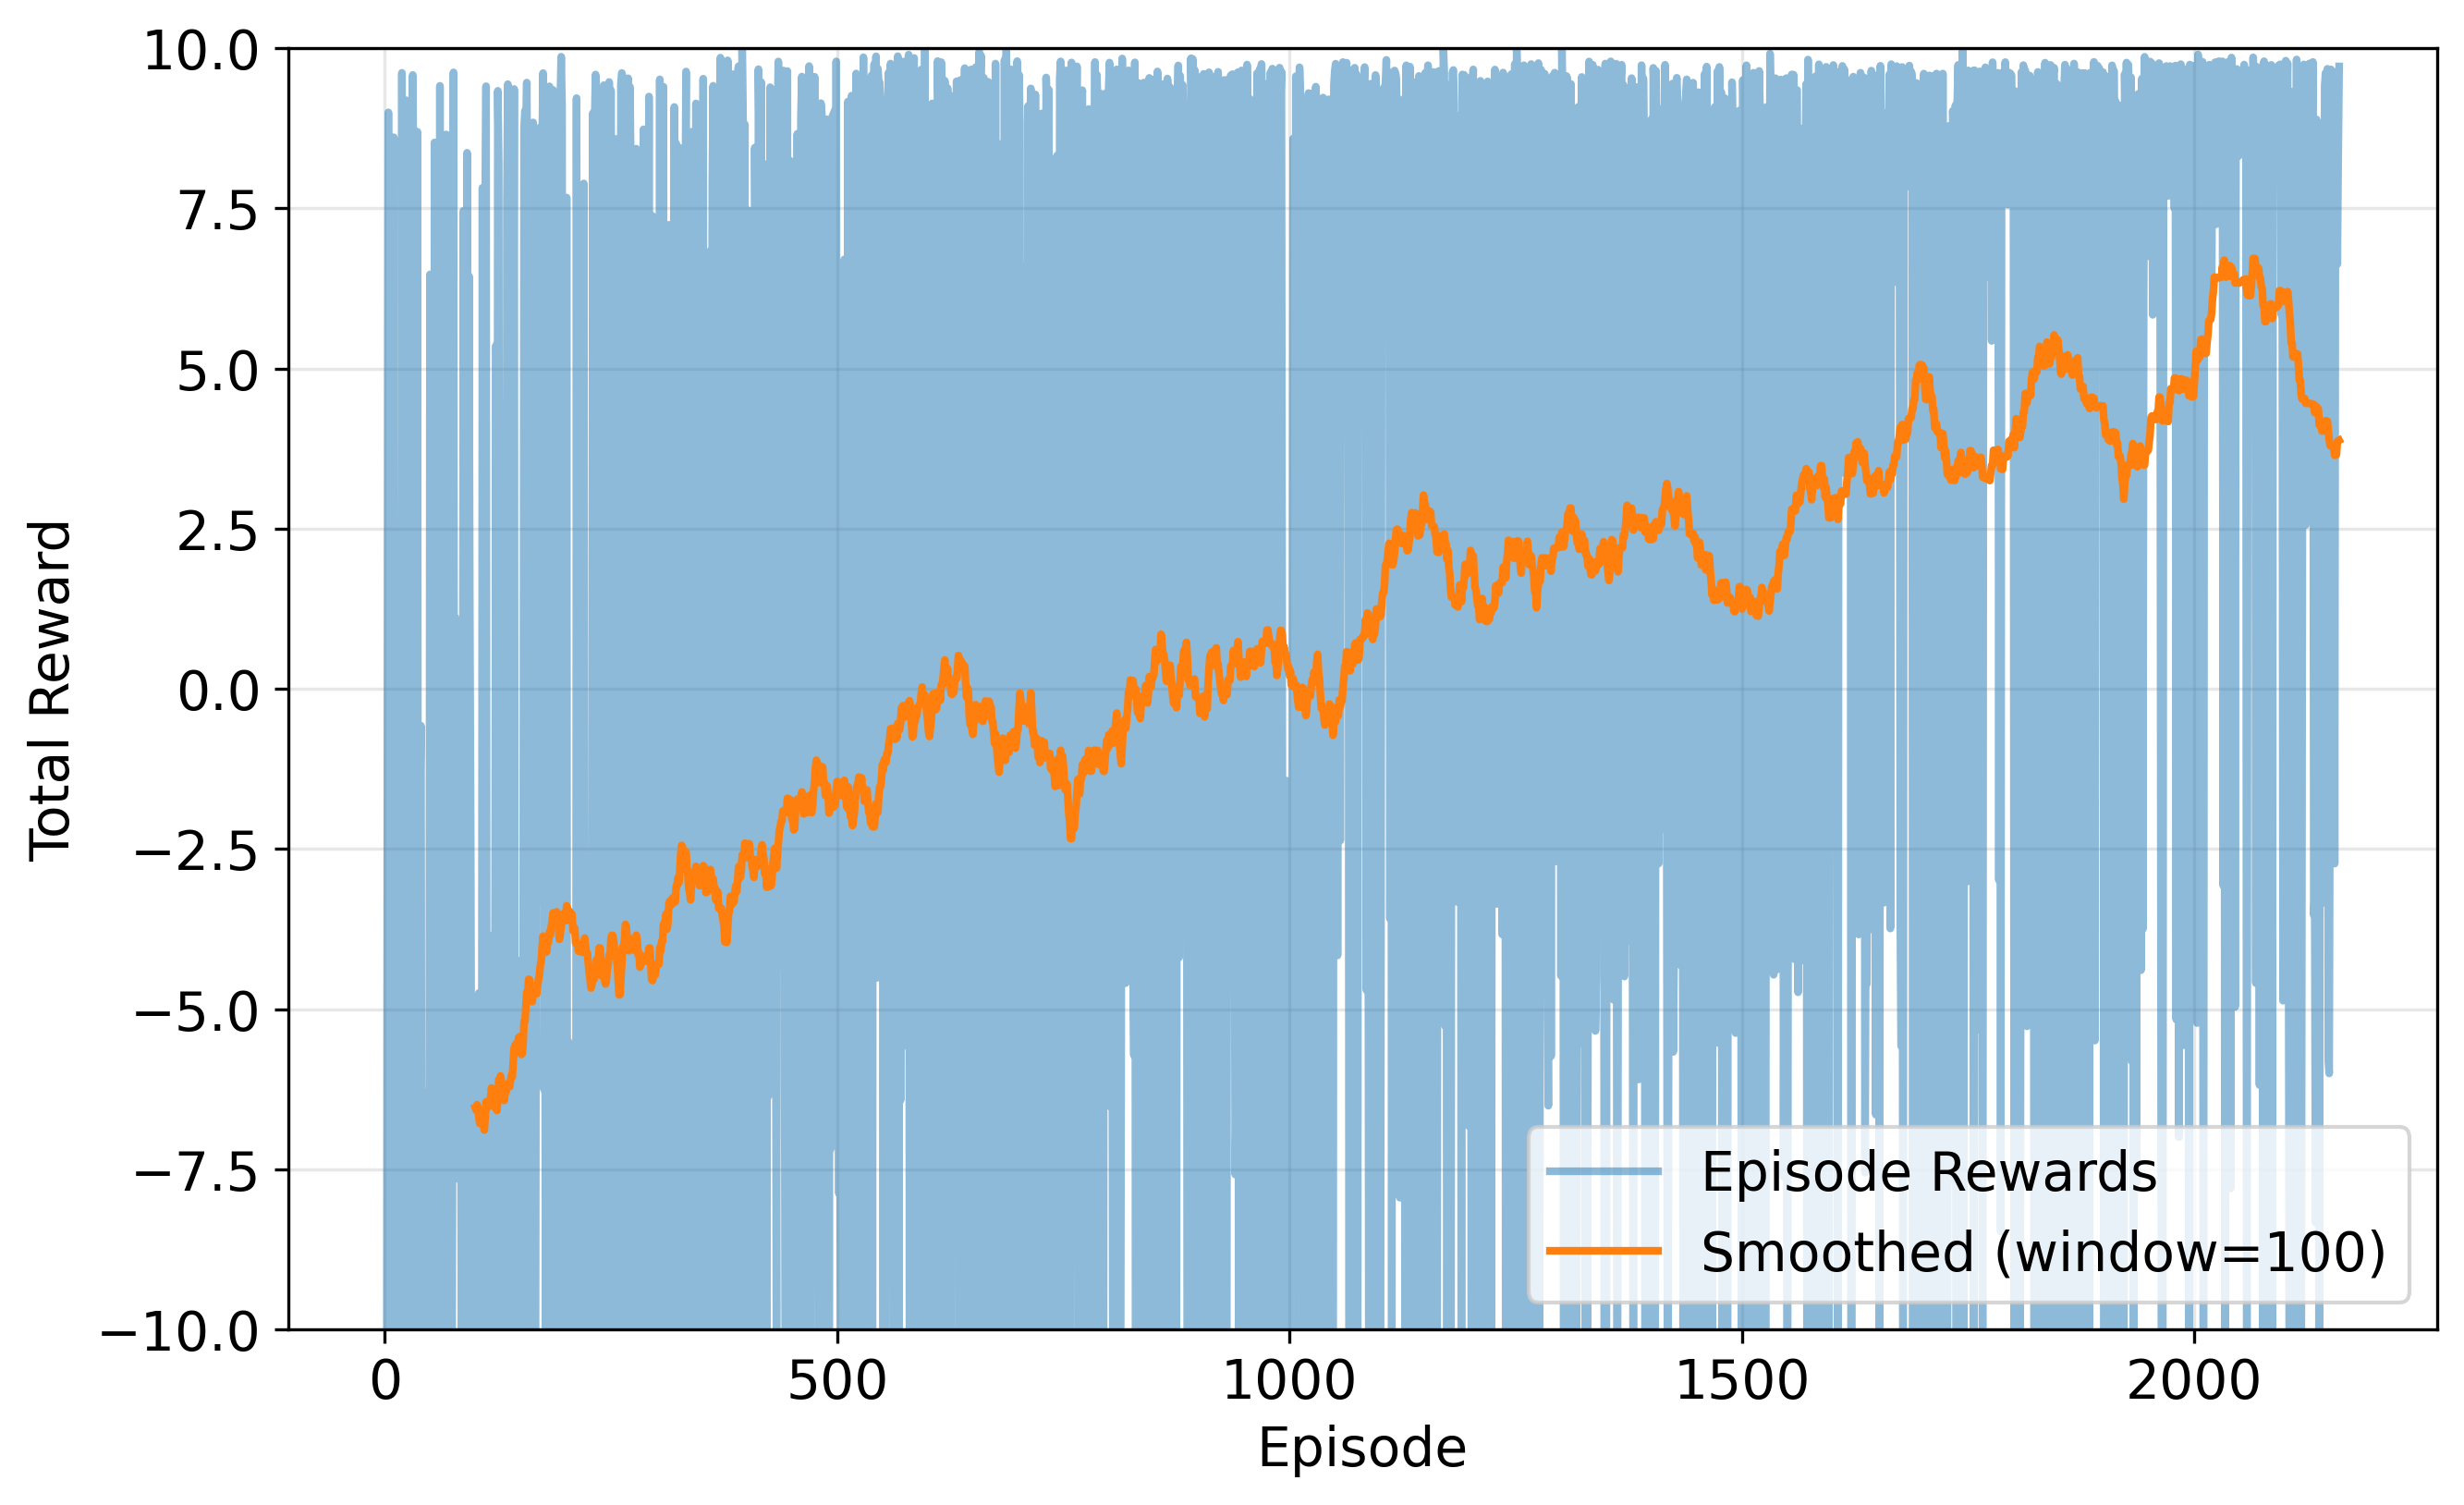
\includegraphics[width=0.5\textwidth]{plots/episode_rewards_sac.png}\label{fig:rewards_sac}}
    \hspace{0.5cm} % Adds horizontal space between the two images
    \subfloat[Winrate vs BasicOpponent-strong across 100 matches]{\includegraphics[width=0.4\textwidth]{plots/winrate_sac.pdf}\label{fig:wins_sac}}
    \caption{Performance of SAC in hockey-env}
    \label{fig:SAC-perf}
\end{figure}
The SAC agent's performance critically depends on the diversity of training experiences. Due to a bug in our self-play mechanism, most SAC training runs (SAC-vs-SAC, SAC-vs-Rainbow, or SAC-vs-TDMPC) were ineffective because we failed to mirror the opponent’s state space appropriately. After fixing this issue for the competition, the SAC agent was primarily trained against the strong bot, and it exploited this opponent’s predictable flaw of leaving its goal unguarded while aggressively controlling the center. Consequently, the SAC agent learned to score with angled, wall-bouncing shots.
